\chapter{Phương pháp nghiên cứu}
\section{Cơ sở lý thuyết}
Hệ thống phân loại màu sắc hoạt động chủ yếu dựa trên hai nguyên tắc điều khiển cốt lõi: Mô hình Máy trạng thái hữu hạn (Finite State Machine - FSM ) để quản lý các trạng thái của hệ thống cũng như luồng logic, và Bộ điều khiển PID giúp tối ưu hóa tốc độ động cơ DC. Ngoài ra, hệ thống còn tích hợp các phần cứng chuyên dụng như (cảm biến, động cơ DC, servo và băng tải). Sự phối hợp nhằm đảm bảo sự ổn định toàn hệ thống và đạt hiệu suất hoạt động cao và chính xác nhất. 

\subsection{Thiết kế Finite State Machine (FSM)}
\subsubsection{Tổng quan về FSM}
Máy trạng thái hữu hạn (Finite State Machine – FSM) là một mô hình trừu tượng dùng để biểu diễn hoạt động của một hệ thống chỉ có thể tồn tại trong một số hữu hạn các trạng thái. Ở mỗi trạng thái, hệ thống tạo ra một hoặc nhiều tín hiệu đầu ra, và khi xảy ra một sự kiện nhất định, nó sẽ chuyển từ trạng thái này sang trạng thái khác. Việc lựa chọn trạng thái kế tiếp có thể phụ thuộc vào các tín hiệu đầu vào. Xét về bản chất, FSM thể hiện chức năng tương tự như cách một chương trình hay một máy tính vận hành và xử lý thông tin.\\
FSM có hai kiến trúc phổ biến là Moore và Mealy. Ở kiến trúc Moore, các tín hiệu đầu ra chỉ phụ thuộc vào trạng thái hiện tại của hệ thống, còn trạng thái kế tiếp được xác định dựa trên trạng thái hiện tại kết hợp với các tín hiệu đầu vào. Trong khi đó, ở kiến trúc Mealy, các tín hiệu đầu ra phụ thuộc đồng thời vào trạng thái hiện tại và các tín hiệu đầu vào, và trạng thái kế tiếp cũng là hàm của trạng thái hiện tại và đầu vào. Sự khác biệt này tạo nên đặc điểm riêng về cách hoạt động và thiết kế của mỗi loại FSM\cite{lewis2013finite}.\\
\subsubsection{Thiết kế FSM}
%\begin{figure}[h] % h: tại đây, t: đầu trang, b: cuối trang, p: trang riêng
%   \centering
%    \includegraphics[width=0.8\textwidth]{} 
%   \caption{Thiết kế FSM theo kiến trúc Moore.} % Chú thích ảnh
%    \label{fig:fsm_moore_diagram} % Nhãn để trích dẫn trong bài
%\end{figure}
\subsubsection*{Bảng trạng thái:}
% Bảng 1: Bảng chuyển trạng thái FSM
\begin{table}[htbp]
    \centering
    
    \begin{tabular}{|l|l|l|l|}
        \hline
        \textbf{Current State} & \multicolumn{1}{c|}{\textbf{Input}} & \multicolumn{1}{c|}{\textbf{Output}} & \textbf{Next State} \\ \hline
        S0 & BTN\_START & xTaskNotify(rgb\_task) & S1 \\ 
           &            & is\_running=true       &    \\ \hline
        S0 & BTN\_SPEED & speed\_idx++           & S1 \\ \hline
        S1 & CLASSIFY\_DONE & servo\_open/close() & S2 \\ 
           &                & motor\_set\_speed() &    \\ \hline
        S2 & IR\_DETECTED   & motor\_set\_speed(0) & S0 \\ 
           &                & counter[color]++    &    \\ 
           &                & is\_running=false    &    \\ \hline
        S2 & TIMEOUT        & motor\_set\_speed(0) & S0 \\ 
           &                & is\_running=false    &    \\ \hline
    \end{tabular}
    \vspace{0.3cm}
    \caption{Bảng các trạng thái của FSM}
\end{table}
\newpage
\noindent \textbf{Encoding} % Chữ Encoding nằm ngoài bảng

% Bảng 2: Bảng giải thích trạng thái
\begin{table}[htbp]
    \centering
    \begin{tabular}{|p{4cm}|p{6cm}|}
        \hline
        \multicolumn{1}{|c|}{\textbf{State}} & \multicolumn{1}{c|}{\textbf{Action}} \\ \hline
        S0 & IDLE \\ \hline
        S1 & CLASSIFYING \\ \hline
        S2 & COVEYOR\_RUNNING \\ \hline
    \end{tabular}
    \vspace{0.3cm} % Tạo khoảng cách nhỏ giữa bảng và caption
    \caption{Bảng Encoding} % Dùng caption* để tự định nghĩa số thủ công giống ảnh
\end{table}

\subsubsection{Các trạng thái của FSM}
FSM của hệ thống bao gồm ba trạng thái chính: IDLE, CLASSIFYING và CONVEYOR\_RUNNING.\\
% Đoạn văn bản mô tả trạng thái IDLE
\textbf{Trạng thái IDLE} là trạng thái chờ của hệ thống. Khi ở trạng thái này, băng tải dừng hoạt động và biến $is\_running$ được đặt bằng 0, biểu thị rằng hệ thống không thực hiện chu trình phân loại nào. Hệ thống chờ tín hiệu từ người dùng thông qua các nút nhấn. 

Khi nhận được tín hiệu khởi động ($BTN\_START$), hệ thống gửi tín hiệu thông báo (notify) đến tác vụ $rgb\_task$, đồng thời đặt $is\_running$ = 1 để khóa việc kích hoạt lặp lại và chuyển sang trạng thái CLASSIFYING. Trong khi đó, tín hiệu thay đổi tốc độ ($BTN\_SPEED$) chỉ làm thay đổi tham số điều khiển thông qua biến $speed\_idx$ và mảng $speed\_buffer[]$, không làm thay đổi trạng thái FSM.\\

\textbf{Trạng thái CLASSIFYING} là giai đoạn hệ thống thực hiện nhận diện màu sắc của sản phẩm. Trong trạng thái này, tác vụ $rgb\_task$ được kích hoạt để đọc dữ liệu từ cảm biến màu và xác định màu chủ đạo thông qua phương pháp bỏ phiếu nhằm đảm bảo độ ổn định của kết quả. Dựa trên màu sắc nhận được, các cơ cấu chấp hành được điều khiển để định hướng phân loại sản phẩm. Sau khi quá trình nhận diện và điều khiển servo hoàn tất, hệ thống phát sinh sự kiện nội bộ CLASSIFY\_DONE và chuyển sang trạng thái CONVEYOR\_RUNNING.\\

\textbf{Trạng thái CONVEYOR\_RUNNING} là giai đoạn băng tải hoạt động để vận chuyển sản phẩm đến vị trí phân loại. Động cơ băng tải được điều khiển bằng bộ PID nhằm duy trì tốc độ ổn định theo giá trị đã chọn. Trong suốt trạng thái này, hệ thống liên tục giám sát các cảm biến hồng ngoại. Khi cảm biến phát hiện sản phẩm ($IR\_DETECTED$) hoặc khi xảy ra quá thời gian cho phép ($TIMEOUT$), băng tải được dừng lại, bộ đếm sản phẩm theo màu ($counter[color]$) được cập nhật, biến $is\_running$ được đặt về 0 và FSM quay trở lại trạng thái IDLE để sẵn sàng cho chu kỳ phân loại tiếp theo.\\
Các tín hiệu đầu vào đóng vai trò kích hoạt chuyển trạng thái bao gồm:
\begin{itemize}
    \item BTN\_START: Nút nhấn khởi động chu trình phân loại.
    \item BTN\_SPEED: Nút nhấn thay đổi tốc độ băng tải.
    \item CLASSIFY\_DONE: Sự kiện nội bộ báo hiệu hoàn tất quá trình nhận diện màu.
    \item IR\_DETECTED: Sự kiện phát sinh khi cảm biến hồng ngoại phát hiện sản phẩm.
    \item TIMEOUT: Sự kiện bảo vệ khi băng tải chạy quá thời gian cho phép.
\end{itemize}

\subsection{Thiết kế Bộ điều khiển PID cho DC motor}
\subsubsection{Tổng quan về DC motor}
Động cơ DC được lựa chọn cho hệ thống băng chuyền vì có cấu trúc đơn giản, dễ điều khiển tốc độ và đáp ứng nhanh với sự thay đổi tải. Tốc độ của động cơ DC có thể điều chỉnh trực tiếp thông qua điện áp hoặc độ rộng xung PWM, giúp việc điều khiển băng chuyền trở nên linh hoạt và chính xác. So với các loại động cơ khác như động cơ AC hay động cơ bước, động cơ DC có chi phí thấp, dễ tích hợp với vi điều khiển và đủ mô-men xoắn cho các hệ thống băng chuyền quy mô nhỏ và trung bình.\\
Bộ điều khiển PID đặc biệt hiệu quả khi áp dụng cho động cơ DC do đặc tính động học gần tuyến tính và mô hình điều khiển đơn giản của loại động cơ này. Mối quan hệ trực tiếp giữa tín hiệu điều khiển và tốc độ giúp PID dễ tinh chỉnh và đạt hiệu quả cao trong việc duy trì tốc độ ổn định. Trong khi đó, các loại động cơ khác thường có đặc tính phi tuyến hoặc đã tích hợp sẵn bộ điều khiển nội bộ, khiến việc áp dụng PID trực tiếp kém hiệu quả hoặc không cần thiết.
\textbf{Phần cứng sử dụng: }
\begin{figure}[htbp] % h: tại đây, t: đầu trang, b: cuối trang, p: trang riêng
  \centering 
    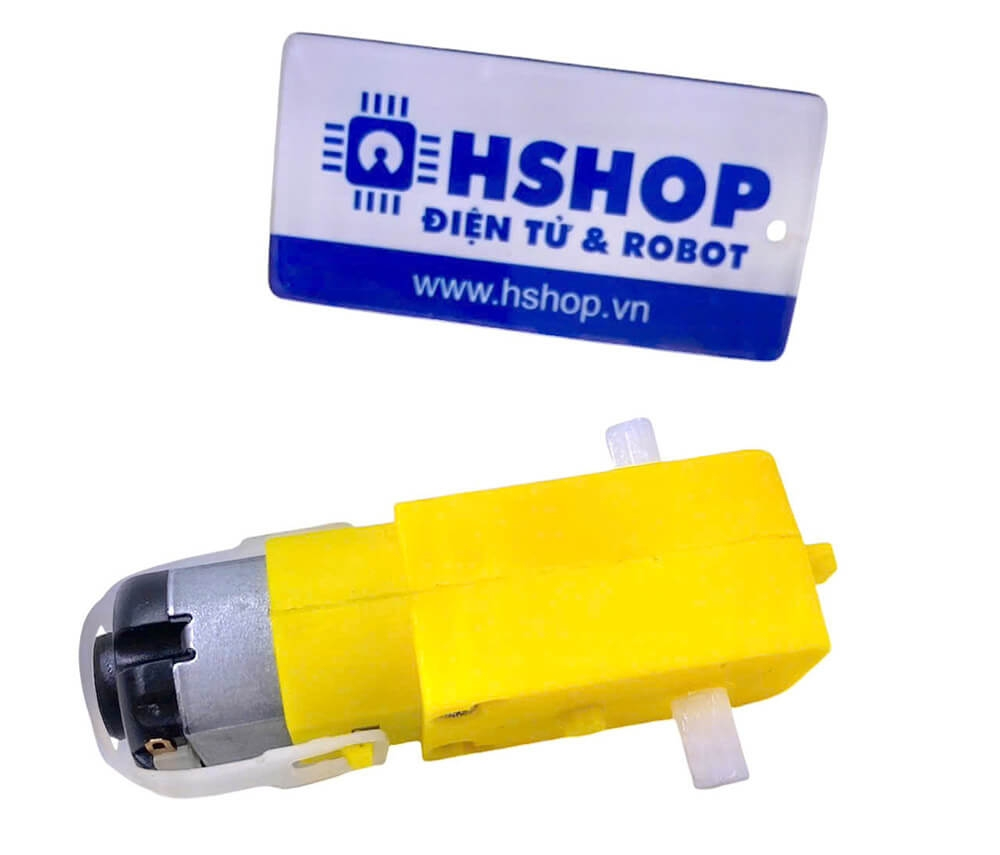
\includegraphics[width=0.8\textwidth]{imgs/dcmotor} 
   \caption{ Động cơ DC giảm tốc V1 Dual Shaft Plastic Geared TT Motor} % Chú thích ảnh
    \label{fig:dc_motor} % Nhãn để trích dẫn trong bài
\end{figure}

Động cơ DC giảm tốc V1 Dual Shaft Plastic Geared TT Motor là loại được lựa chọn và sử dụng nhiều nhất hiện nay cho các thiết kế khung Robot, xe, thuyền,... , động cơ có chất lượng và giá thành vừa phải cùng với khả năng dễ lắp ráp đem đến chi phí tiết kiệm và sự tiện dụng cho người sử dụng\cite{hshop_motor_dc}. Vì thế nhóm chọn động cơ này cho băng chuyền quy mô nhỏ với phân loại hàng hóa nhẹ không cần sức kéo mạnh.Ngoài ra động cơ còn kết hợp được với bánh đĩa 20 xung phục vụ cho quá trình encoder lấy dữ liệu tốc độ phục vụ cho thiết kế Bộ điều khiển PID.


\subsubsection{Tổng quan về H-brigde}
Tuy nhiên, để điều khiển được động cơ DC, không thể cấp trực tiếp nguồn từ vi xử lý vào động cơ do khả năng cấp dòng của vi xử lý rất nhỏ, không đáp ứng được yêu cầu công suất của động cơ. Vì vậy, cần sử dụng mạch H-bridge làm tầng khuếch đại công suất trung gian. H-bridge cho phép vi xử lý đưa tín hiệu điều khiển dạng xung PWM vào mạch công suất, từ đó mạch sẽ cung cấp dòng điện và điện áp phù hợp cho động cơ DC, đồng thời cho phép điều khiển tốc độ và chiều quay một cách linh hoạt và hiệu quả.\\
Mạch cầu H là một mạch điện cơ bản dùng để điều khiển động cơ DC quay thuận hoặc quay nghịch bằng cách thay đổi chiều dòng điện cấp vào động cơ. Trong thực tế, mạch cầu H có nhiều cấu hình khác nhau tùy thuộc vào việc lựa chọn linh kiện công suất, khả năng chịu dòng và điện áp, cũng như tần số xung PWM sử dụng, từ đó quyết định hiệu năng và khả năng điều khiển của mạch. Nguyên lý hoạt động của mạch dựa trên đặc tính của động cơ DC: khi đảo chiều dòng điện chạy qua động cơ thì chiều quay của động cơ cũng thay đổi tương ứng. Vì vậy, bằng cách điều khiển các khóa trong mạch cầu H để đổi chiều cấp điện, có thể điều khiển linh hoạt chiều quay và tốc độ của động cơ.\\
\textbf{Phần cứng sử dụng:}
\begin{figure}[htbp] % h: tại đây, t: đầu trang, b: cuối trang, p: trang riêng
  \centering
    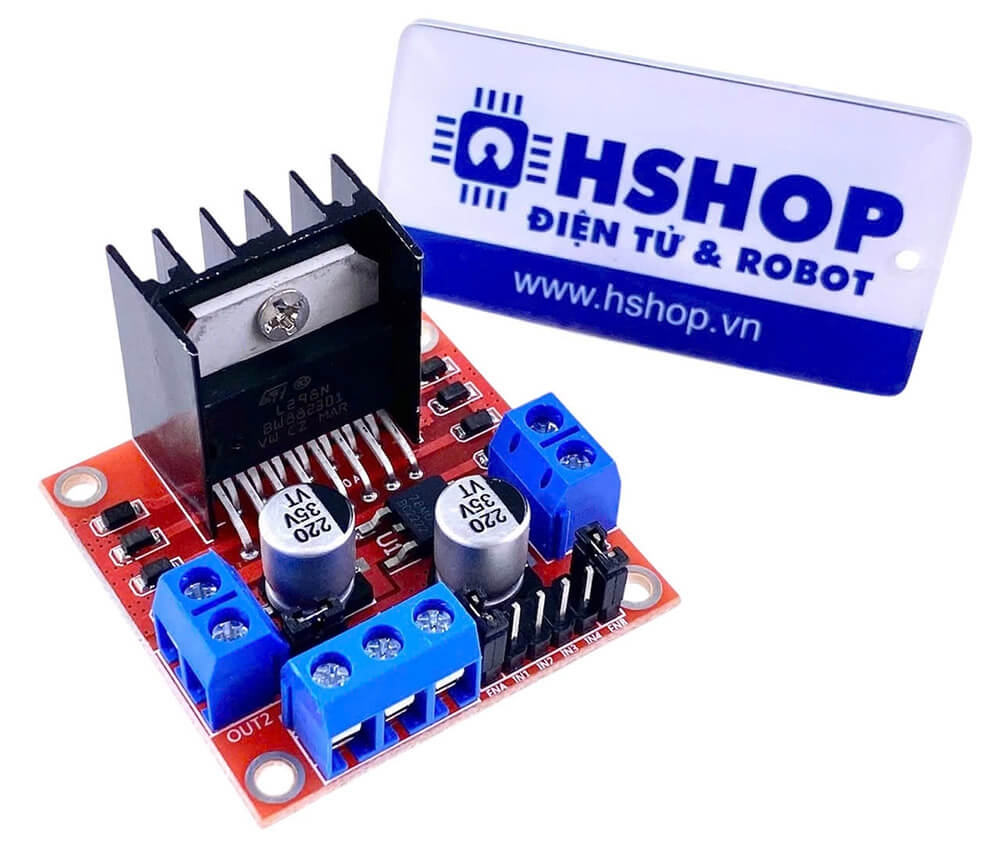
\includegraphics[width=0.8\textwidth]{imgs/l298n} 
   \caption{ Mạch điều khiển động cơ L298 DC Motor Driver\cite{hshop_l298}} % Chú thích ảnh
    \label{fig:h_brigde_l298n} % Nhãn để trích dẫn trong bài
\end{figure}
L298 là mạch điều khiển động cơ tích hợp hai cầu H độc lập, cho phép điều khiển linh hoạt hai động cơ DC hoặc một động cơ bước. Mỗi cầu H có khả năng đảo chiều dòng điện để điều khiển chiều quay thuận và nghịch của động cơ, đồng thời có thể kết hợp với tín hiệu PWM để điều chỉnh tốc độ. Mạch L298 DC Motor Driver hỗ trợ dòng tải lên đến khoảng 2 A cho mỗi kênh, được tích hợp diode bảo vệ chống dòng ngược và IC ổn áp 7805 để cung cấp nguồn 5 VDC cho các module điều khiển. Nhờ cấu trúc hai cầu H và khả năng làm việc ổn định, L298 được sử dụng phổ biến trong các hệ thống điều khiển động cơ DC và động cơ bước.
\subsubsection{Tổng quan về PID}

\subsection{Các phần cứng chuyên dụng}
\subsubsection{Tổng quan về Color Sensor}
Cảm biến màu (color sensor) là một thiết bị quang điện dùng để đo lường và nhận diện màu sắc của vật thể thông qua việc phân tích ánh sáng phản xạ từ bề mặt của nó. Cảm biến thường chiếu ánh sáng lên vật thể, sau đó thu nhận ánh sáng phản xạ và xác định cường độ của các thành phần màu cơ bản như đỏ (R), xanh lá (G) và xanh dương (B). Nhờ đó, cảm biến có thể suy ra màu sắc tổng thể của vật thể. Cảm biến màu được ứng dụng rộng rãi trong các lĩnh vực như robot, tự động hóa công nghiệp, y tế và các hệ thống IoT.\\
Nguyên lý hoạt động của cảm biến màu dựa trên quá trình phân tích ánh sáng. Ánh sáng từ nguồn chiếu lên vật thể sẽ bị phản xạ hoặc truyền qua và đi vào cảm biến. Bên trong cảm biến có các bộ lọc màu hoặc mảng cảm biến quang học tương ứng với các kênh RGB, mỗi kênh có nhiệm vụ đo cường độ ánh sáng của một màu cơ bản. Các giá trị R, G và B thu được sẽ được vi xử lý trong cảm biến hoặc trong hệ thống điều khiển tổng hợp và xử lý để xác định màu sắc của vật thể.
\textbf{Phần cứng sử dụng:}
\begin{figure}[htbp] % h: tại đây, t: đầu trang, b: cuối trang, p: trang riêng
  \centering
    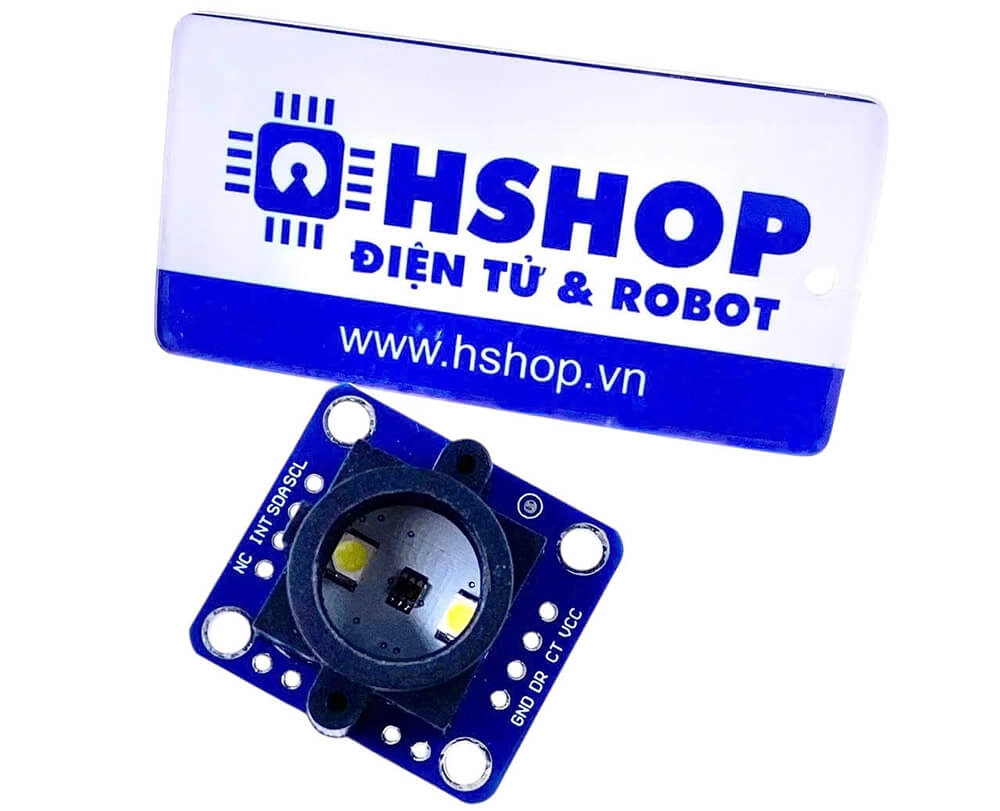
\includegraphics[width=0.8\textwidth]{imgs/tsc34725} 
   \caption{  Cảm biến màu sắc I2C UART TCS34725 Color Sensor V1\cite{hshop_tcs34725}} % Chú thích ảnh
    \label{fig:color_Sensor} % Nhãn để trích dẫn trong bài
\end{figure}
Cảm biến màu TCS34725 sử dụng chip TCS34725, cho phép đo và xuất trực tiếp các giá trị màu RGB thông qua giao tiếp I2C (và một số mô-đun hỗ trợ thêm UART). Cảm biến có thể được sử dụng dưới dạng mô-đun đơn giản hoặc kết hợp với vi điều khiển để đọc và xử lý dữ liệu màu. Trong một số cấu hình, MCU nội bộ có thể thực hiện việc cân bằng trắng và xuất trực tiếp giá trị RGB, giúp giảm tải cho hệ thống điều khiển trung tâm. Nhờ khả năng giao tiếp linh hoạt và dữ liệu đầu ra trực tiếp, TCS34725 dễ dàng tích hợp vào các hệ thống nhúng.\\
Việc sử dụng TCS34725 mang lại nhiều lợi ích cho hệ thống phân loại màu. Cảm biến được tích hợp bộ lọc chặn hồng ngoại (IR filter), giúp giảm ảnh hưởng của thành phần quang phổ IR trong ánh sáng môi trường, từ đó nâng cao độ chính xác của phép đo màu. Ngoài ra, TCS34725 có khả năng xuất dữ liệu RGB ổn định mà không cần thực hiện cân bằng trắng phức tạp ở mức ứng dụng, giúp đơn giản hóa thuật toán xử lý và tăng độ tin cậy của hệ thống. Những đặc điểm này khiến TCS34725 trở thành lựa chọn phù hợp cho các ứng dụng nhận diện màu trong robot và hệ thống tự động hóa.
\subsubsection{Tổng quan về Encoder}
Trong các hệ thống điều khiển động cơ DC, vi xử lý chỉ có khả năng phát xung điều khiển (như PWM) để điều chỉnh tốc độ hoặc hướng quay, nhưng không thể trực tiếp nhận biết các thông tin phản hồi về trạng thái hoạt động thực tế của động cơ như vị trí, số vòng quay hay tốc độ. Do đó, encoder trở thành phần tử phản hồi quan trọng, giúp cung cấp dữ liệu cần thiết để vi xử lý giám sát và điều khiển động cơ chính xác hơn, đồng thời hình thành hệ thống điều khiển vòng kín nhằm tăng độ ổn định và khả năng bù sai lệch trong quá trình vận hành.\\
Encoder hoạt động dựa trên nguyên lý đĩa mã hóa quay quanh trục động cơ, trên đĩa có các rãnh cho phép ánh sáng từ nguồn phát xuyên qua. Khi đĩa quay, cảm biến quang sẽ luân phiên ghi nhận trạng thái có hoặc không có ánh sáng, từ đó tạo ra chuỗi xung vuông. Số xung thu được phản ánh vị trí hoặc số vòng quay, trong khi tần số xung cho biết tốc độ của động cơ. Các tín hiệu xung này được truyền về bộ xử lý trung tâm như vi xử lý hoặc PLC để phục vụ cho việc giám sát và điều khiển.
\textbf{Phần cứng sử dụng:}
\begin{figure}[h] % h: tại đây, t: đầu trang, b: cuối trang, p: trang riêng
  \centering
    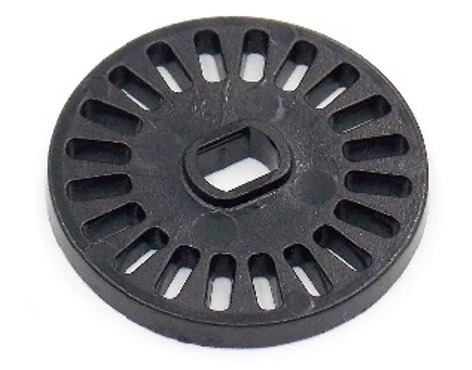
\includegraphics[width=0.8\textwidth]{imgs/encoder} 
   \caption{  Đĩa Encoder 20 xung \cite{hshop_encoder_dia}} % Chú thích ảnh
    \label{fig:encoder} % Nhãn để trích dẫn trong bài
\end{figure}
\begin{figure}[htbp] % h: tại đây, t: đầu trang, b: cuối trang, p: trang riêng
  \centering
    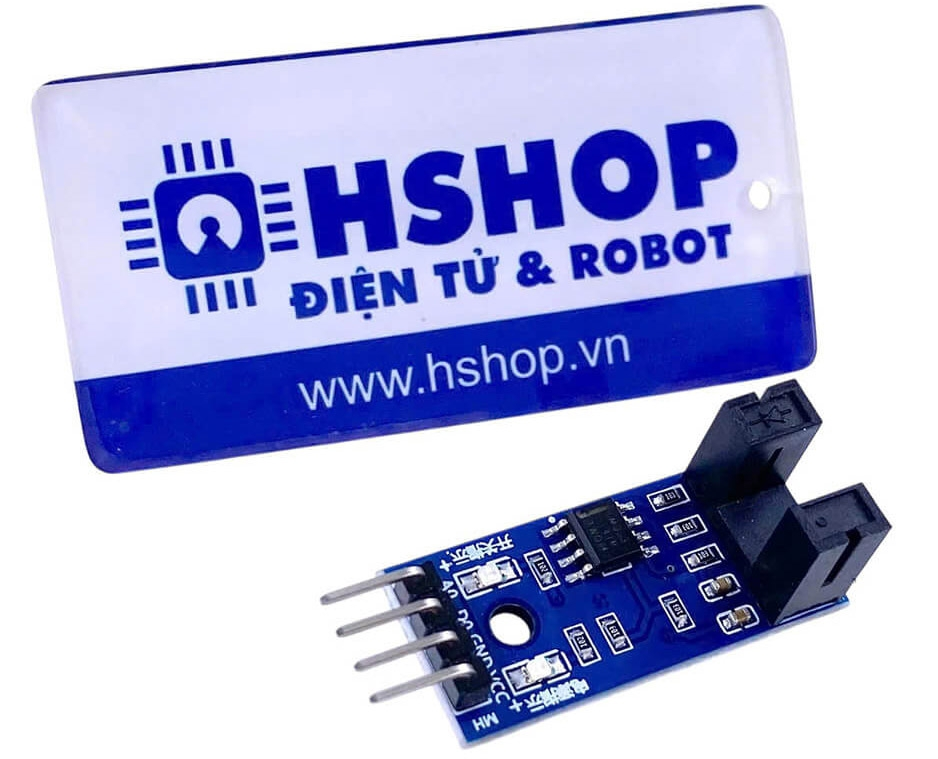
\includegraphics[width=0.8\textwidth]{imgs/cambientocdo} 
   \caption{  Mạch cảm biến tốc độ Encoder V1\cite{hshop_encoder_module}} % Chú thích ảnh
    \label{fig:encoder_module} % Nhãn để trích dẫn trong bài
\end{figure}
Mạch cảm biến tốc độ Encoder V1 bao gồm 1 mắt phát và 1 mắt thu hồng ngoại đặt cách nhau qua 1 khe hở, khi ánh sáng từ mắt phát đi được tới mắt thu (xuyên qua lỗ của dĩa encoder) thì sẽ có tín hiệu mức cao (5v) phát ra khỏi chân out, khi bị che lại thì chân out phát ra tín hiệu mức thấp (0v). Encoder V1 và đĩa Encoder 20 xung được thiết kế phù hợp để tương thích với Động Cơ DC Giảm Tốc V1 Dual Shaft Plastic Geared TT Motor.
